% !TEX program = xelatex
\documentclass[12pt]{article}
\usepackage[a4paper, margin=2.45cm]{geometry}
\usepackage[fleqn]{amsmath}
\usepackage{amssymb}
\usepackage{amsfonts}
\usepackage[dvipsnames]{xcolor}
\usepackage{setspace}
\usepackage{graphicx}
\usepackage{cancel}
\usepackage{xfrac}
\usepackage{fontenc}
\usepackage{fontspec}
\usepackage[none]{hyphenat}
\usepackage{etoolbox}
\usepackage{longtable}
\usepackage{listings}
\usepackage{listings-rust}

\setlength{\LTleft}{0pt}
\lstset{basicstyle = \footnotesize\color{white}\ttfamily, backgroundcolor = \color{bg}}
\AtBeginEnvironment{align}{\setcounter{equation}{0}}
\setmonofont{Consolas}
\everymath{\displaystyle}
\begin{document}
% \onehalfspacing
\definecolor{bg}{gray}{0.1}
% \definecolor{codegreen}{rgb}{0,0.6,0}
% \definecolor{codegray}{rgb}{0.5,0.5,0.5}
% \definecolor{codepurple}{rgb}{0.58,0,0.82}
% \definecolor{backcolour}{rgb}{0.95,0.95,0.92}

% \pagecolor{bg}
% \color{white}
\sloppy
\newcommand{\unt}{\int\displaylimits}
\newcommand{\jadi}{$\therefore\;$}
\newcommand{\rut}[1]{\sqrt{#1}}
\newcommand{\jgj}{\Leftrightarrow}
\newcommand{\tebal}[1]{\underline{\textbf{#1}}\bigskip}
\newcommand{\infak}{\int\displaylimits^{\infty}_{\infty}}
\newcommand{\lqm}{\lim\displaylimits}

\noindent Kelompok 5
\begin{enumerate}
    \item Rafif Rabbani (2102286)
    \item Bagas Ghulam Maulana (2102476)
    \item Muhammad Rahman Wicaksono (2102800)
\end{enumerate}
Pertemuan 3 Analisis Numerik\\
\noindent\rule{\textwidth}{0.2pt}\bigbreak

\begin{enumerate}
    \item {
        Diberikan persamaan sebagai berikut :
        \begin{align*}
            x^2 - 3 - \ln(x) = 0 
        \end{align*}
        Bagaimana metode iterasi titik tetap mencari hampiran akar-akar persamaan tak linier tersebut? \bigskip

        Misalkan diberikan persamaan $ f(x) = 0 $, maka ubah persamaan menjadi bentuk
        \begin{align*}
            (1)\;   & x = g_1(x) \\
            (2)\;   & x = g_2(x) \\
                    & \vdots \\
            (n)\;   & x = g_n(x)
        \end{align*}
        Kemudian diantara fungsi-fungsi tersebut, pilih fungsi $ g(x) $ yang memenuhi
        \begin{align*}
            |g(x)| < 1, \forall x \in [a,b]
        \end{align*}
        untuk suatu selang $ [a,b] $. Lalu pilih titik perkiraan awal $ x_0 \in [a,b]$. Selanjutnya perkiraan akar-akar $ x_n $ dihitung dengan
        \begin{align*}
            x_n = g(x_{n-1})
        \end{align*} 
        Lakukan secara iterasi berulang hingga tingkat galat yang diinginkan tercapai yaitu dengan menghitung
        \begin{align*}
            \left|\frac{x_n - x_{n-1}}{x_n}\right| < \varepsilon
        \end{align*}
        dimana $ \varepsilon $ adalah tingkat galat yang diinginkan.\bigskip

        Untuk kasus $ x^2 - 3 - \ln(x) $, terdapat 2 fungsi yang dapat digunakan yaitu
        \begin{align*}
            (1)\;   & x = g_1(x) = \pm\rut{3 + \ln(x)}  &\\
            (2)\;   & x = g_1(x) = e^{(x^2 - 3)}
        \end{align*}
        Untuk fungsi $ g_1(x) $, diperoleh
        \begin{align*}
            |g_1'(x)| = \left|\pm\dfrac{1}{2x\sqrt{\ln\left(x\right)+3}}\right| = \dfrac{1}{2x\sqrt{\ln\left(x\right)+3}} < 1, \forall x \in (0.356391, \infty)
        \end{align*}
        Kemudian akan digunakan juga metode grafik tunggal untuk menentukan perkiraan akar $ x_0 $
        \begin{center}
            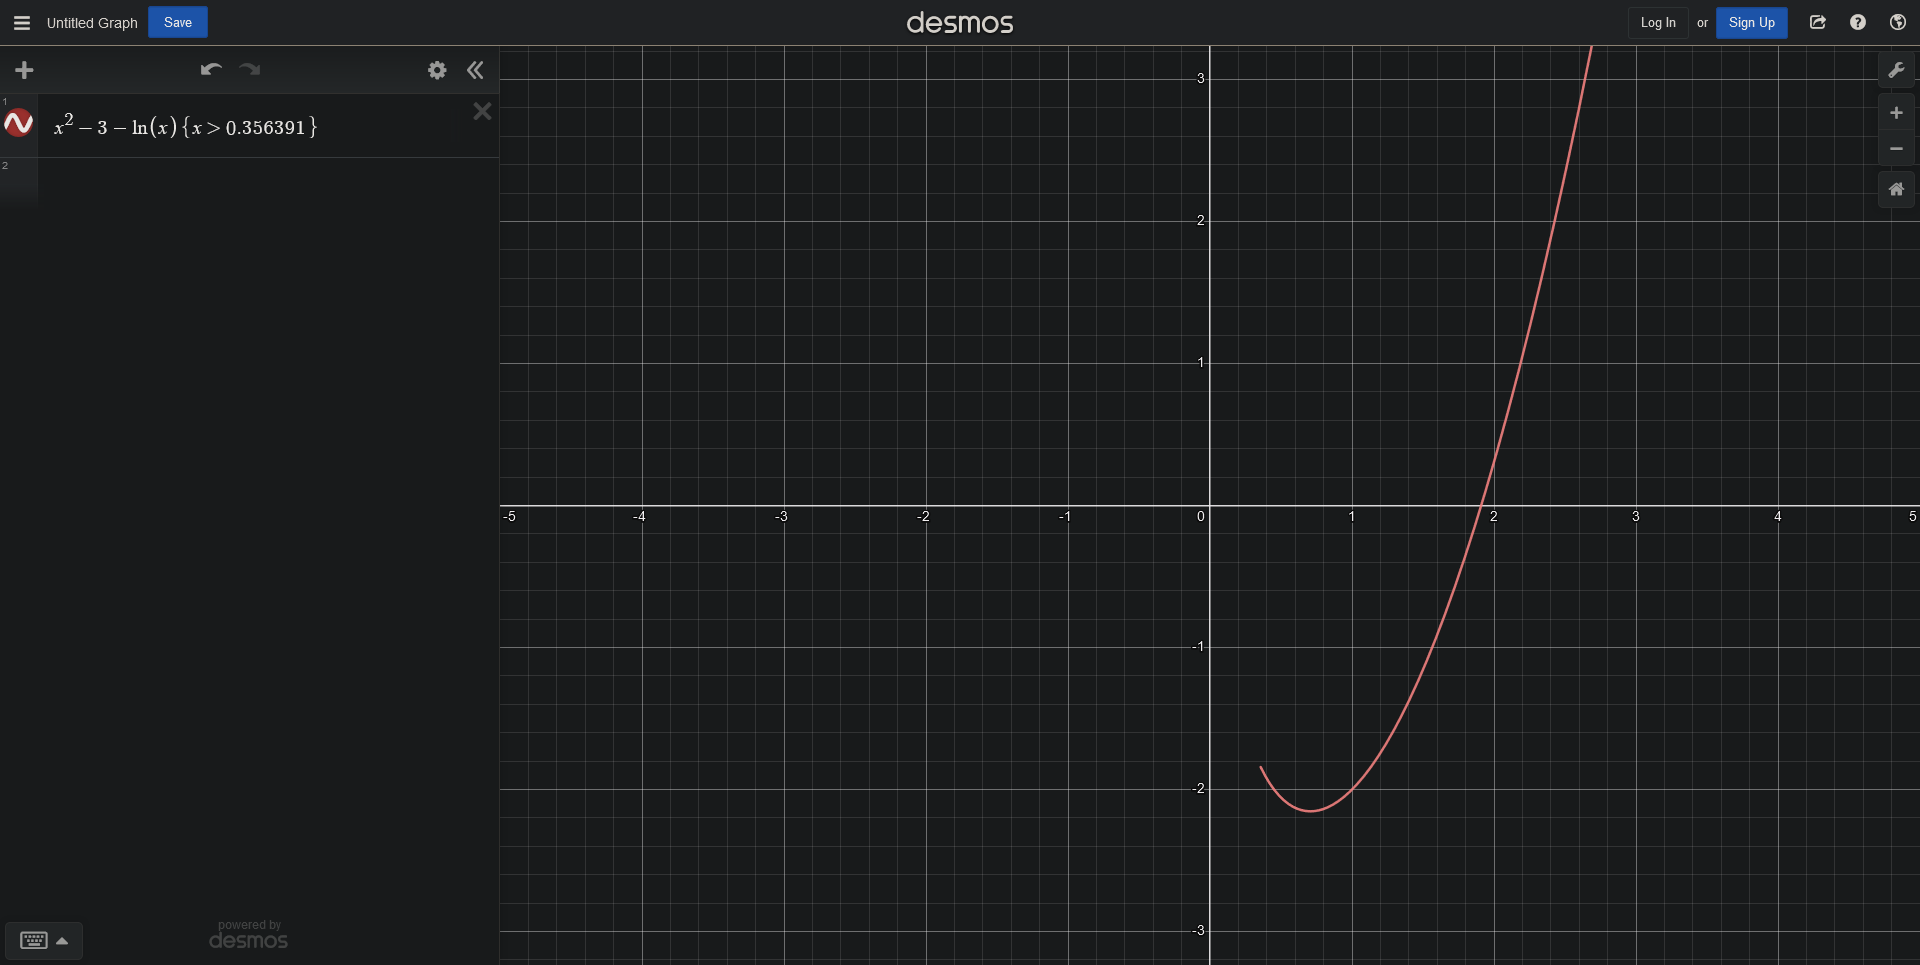
\includegraphics[scale=0.2]{gambar_1.png}  
        \end{center}
        Dari grafik diatas, terlihat bahwa akar sejati terletak di sekitar 1.5. Maka dipilih nilai $ x_0 = 1.5 $. Untuk menghitung hampiran akar-akarnya, akan digunakan bahasa pemograman "Rust" sebagai berikut
        \begin{lstlisting}[language=Rust, style=colouredRust]
    use std::io;

    // INPUT KE VARIABEL
    fn read() -> String {
        let mut buffer = String::new();
        io::stdin()
            .read_line(&mut buffer)
            .expect("Failed");
        return buffer;
    }
    
    // FUNGSI f(x)
    fn f(x:f64) -> f64{
        (x * x) - 3.0 - x.ln() 
    }

    // FUNGSI g(x)
    fn g(x:f64) -> f64 {
        // (x * x - 3.0).exp()
        (3.0 + x.ln()).sqrt()
    }

    // ENTRY POINT
    fn main() {
        
        // INPUT X
        println!();
        println!("x = ");
        let mut x : f64 = read()
            .trim()
            .parse()
            .expect("Failed");

        // UJI PERKIRAAN AWAL
        if f(x) == 0.0 {
            println!();
            println!();
            println!("f(x) = {}", f(x));
            println!();
            println!("Solusi akhir = {x}");
            return ();
        }

        // INPUT GALAT
        println!();
        println!("Batas galat = ");
        let galat : f64 = read()
            .trim()
            .parse()
            .expect("Failed");

        // INPUT BATAS ITERASI
        println!();
        println!("Batas iterasi = ");
        let max : i32 = read()
            .trim()
            .parse()
            .expect("Failed");

        // LOOPING ALGORITMA
        let mut iter = 0;
        while   (true) 
                & (f(g(x)) != 0.0) 
                & ((g(x) - x).abs() > galat) 
                & (iter < max){
            {   // OUTPUT ITERASI
                println!();
                println!();
                println!("Iterasi {iter}");
                println!();
                println!("x{iter} = {x}");
                println!("f(x{iter}) = {}",f(x));
                println!();
                println!("x{} = {}", iter + 1, g(x));
                println!("f(x{}) = {}", iter + 1, f(g(x)));
                println!();
                println!("galat = {}", ((g(x) - x) / g(x)).abs());
            }

            // PERHITUNGAN
            x = g(x);
            iter = iter + 1;
        }
        {   // OUTPUT ITERASI
            println!();
            println!();
            println!("Iterasi {iter}");
            println!();
            println!("x{iter} = {x}");
            println!("f(x{iter}) = {}",f(x));
            println!();
            println!("x{} = {}", iter + 1, g(x));
            println!("f(x{}) = {}", iter + 1, f(g(x)));
            println!();
            println!("galat = {}", ((g(x) - x) / g(x)).abs());
            println!();
            println!();
            println!("Solusi akhir = {x}");
        }
    }
        \end{lstlisting}
        Kemudian perhitungan dilakukan dengan galat sebesar 0.0000001. Diperoleh hasil sebagai berikut
        \begin{lstlisting}
    x =
    1.5
    
    Batas galat =
    0.0000001
    
    Batas iterasi =
    1000
    
    
    Iterasi 0
    
    x0 = 1.5
    f(x0) = -1.1554651081081644
    
    x1 = 1.8453902319314917
    f(x1) = -0.20722565484164668
    
    galat = 0.18716379113483567
    
    
    Iterasi 1
    
    x1 = 1.8453902319314917
    f(x1) = -0.20722565484164668
    
    x2 = 1.9007079636150872
    f(x2) = -0.029535666248805104
    
    galat = 0.029103751203516267
    
    
    Iterasi 2
    
    x2 = 1.9007079636150872
    f(x2) = -0.029535666248805104
    
    x3 = 1.9084617966306312
    f(x3) = -0.004071146319573171
    
    galat = 0.0040628704379795854
    
    
    Iterasi 3
    
    x3 = 1.9084617966306312
    f(x3) = -0.004071146319573171
    
    x4 = 1.9095281028354072
    f(x4) = -0.0005585694360532578
    
    galat = 0.0005584134651868497
    
    
    Iterasi 4
    
    x4 = 1.9095281028354072
    f(x4) = -0.0005585694360532578
    
    x5 = 1.9096743557356166
    f(x5) = -0.00007658818921885135
    
    galat = 0.00007658525641827714
    
    
    Iterasi 5
    
    x5 = 1.9096743557356166
    f(x5) = -0.00007658818921885135
    
    x6 = 1.9096944083133984
    f(x6) = -0.00001050046697304019
    
    galat = 0.00001050041184313098
    
    
    Iterasi 6
    
    x6 = 1.9096944083133984
    f(x6) = -0.00001050046697304019
    
    x7 = 1.9096971575646318
    f(x7) = -0.000001439627849819658
    
    galat = 0.0000014396268133121415
    
    
    Iterasi 7
    
    x7 = 1.9096971575646318
    f(x7) = -0.000001439627849819658
    
    x8 = 1.9096975344902878
    f(x8) = -0.0000001973745508143665
    
    galat = 0.00000019737453141815822
    
    
    Iterasi 8
    
    x8 = 1.9096975344902878
    f(x8) = -0.0000001973745508143665
    
    x9 = 1.9096975861672012
    f(x9) = -0.000000027060260365807665
    
    galat = 0.000000027060260111046353
    
    
    Solusi akhir = 1.9096975344902878
        \end{lstlisting}
        Kemudian dilakukan juga perhitungan menggunakan \emph{software} Microsoft Excel dan diperoleh hasil sebagai berikut
        \begin{center}
            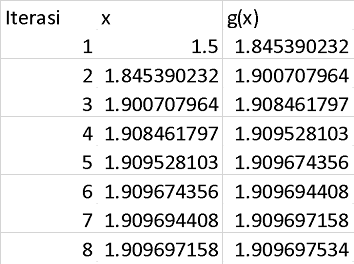
\includegraphics[scale=0.6]{gambar5.png}
        \end{center}
        Diperoleh hasil akhir $ x = 1.9096975344902878 $.\bigskip

        Untuk fungsi $ g_2(x) $, diperoleh
        \begin{align*}
            & |g_2'(x)| < 1 \\
            & \left|2xe^{x^2-3}\right| < 1 \\ 
            & -1 < 2x\mathrm{e}^{x^2-3} < 1 \\
            & -1.40295 < x < 1.40295
        \end{align*}
        Kemudian akan digunakan juga metode grafik tunggal untuk menentukan perkiraan akar $ x_0 $
        \begin{center}
            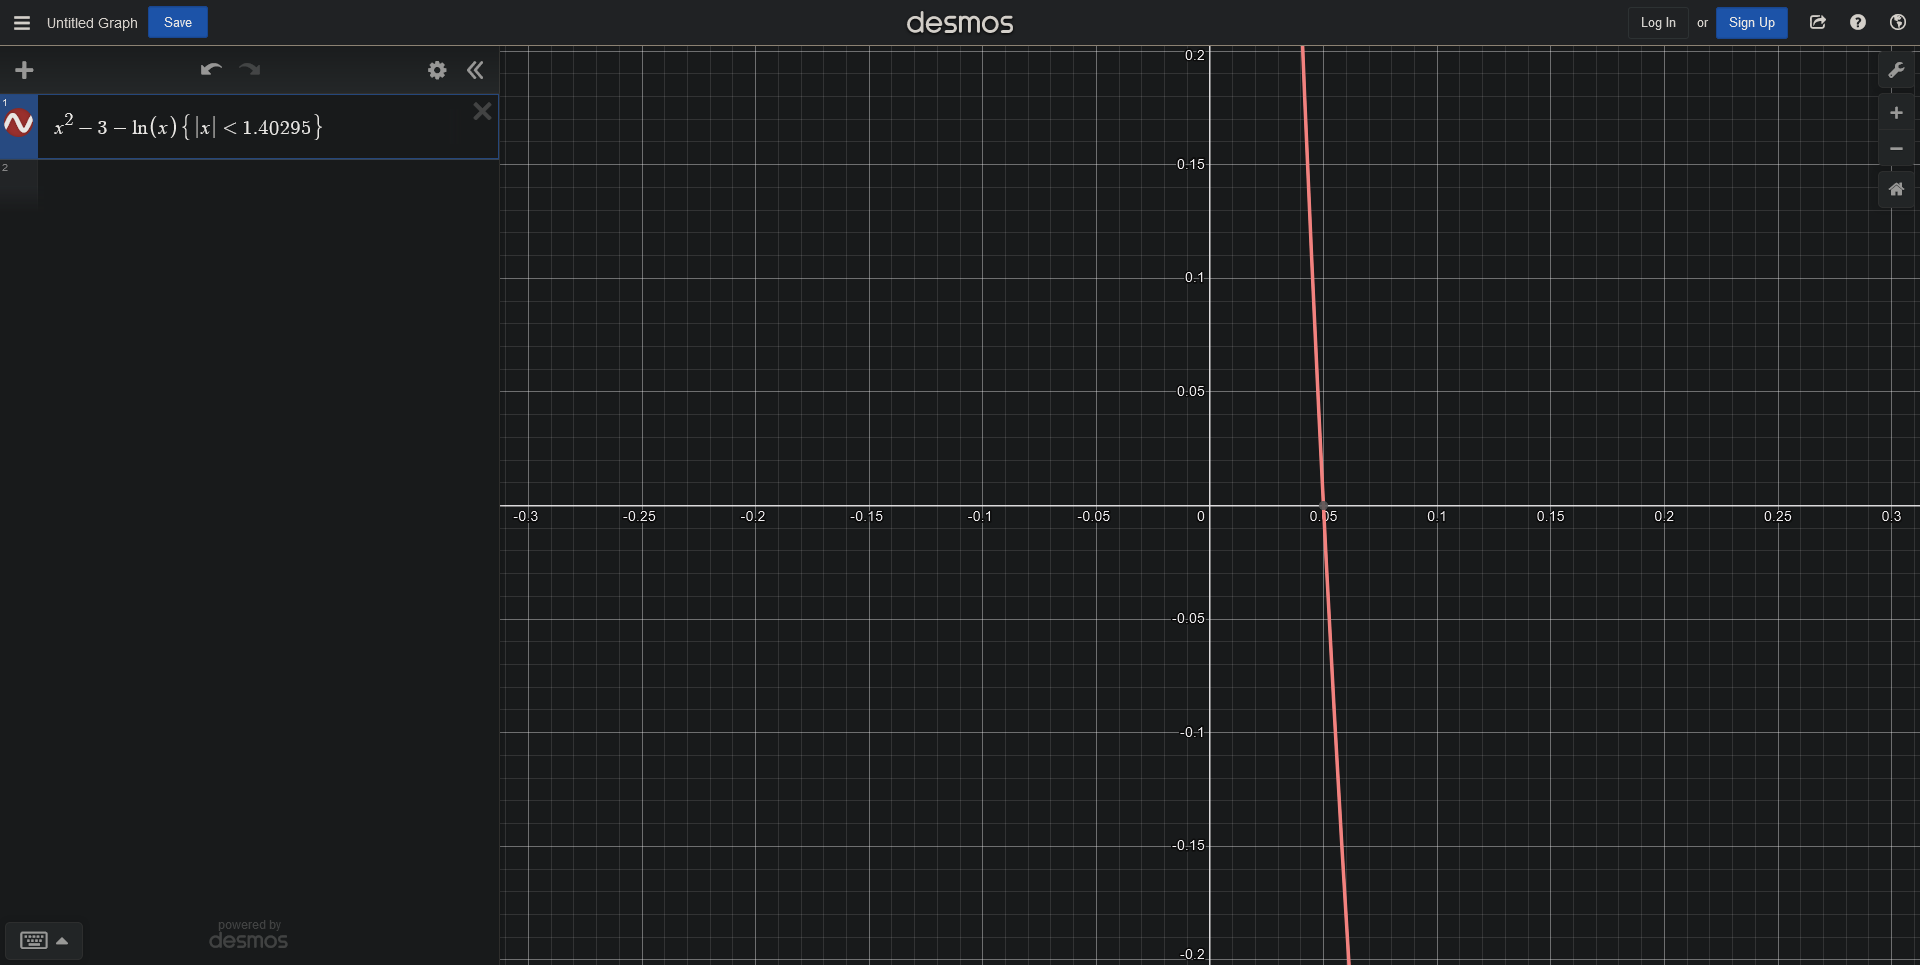
\includegraphics[scale=0.2]{gambar2.png}  
        \end{center}
        Dari grafik diatas, terlihat bahwa akar sejati terletak di sekitar 1. Maka dipilih nilai $ x_0 = 1 $. Untuk menghitung hampiran akar-akarnya, akan digunakan bahasa pemograman "Rust" sebagai berikut
        \begin{lstlisting}[language=Rust, style=colouredRust]
    use std::io;

    // INPUT KE VARIABEL
    fn read() -> String {
        let mut buffer = String::new();
        io::stdin()
            .read_line(&mut buffer)
            .expect("Failed");
        return buffer;
    }

    // FUNGSI f(x)
    fn f(x:f64) -> f64{
        (x * x) - 3.0 - x.ln() 
    }

    // FUNGSI g(x)
    fn g(x:f64) -> f64 {
        (x * x - 3.0).exp()
        // (3.0 + x.ln()).sqrt()
    }

    // ENTRY POINT
    fn main() {
        
        // INPUT X
        println!();
        println!("x = ");
        let mut x : f64 = read()
            .trim()
            .parse()
            .expect("Failed");

        // UJI PERKIRAAN AWAL
        if f(x) == 0.0 {
            println!();
            println!();
            println!("f(x) = {}", f(x));
            println!();
            println!("Solusi akhir = {x}");
            return ();
        }

        // INPUT GALAT
        println!();
        println!("Batas galat = ");
        let galat : f64 = read()
            .trim()
            .parse()
            .expect("Failed");

        // INPUT BATAS ITERASI
        println!();
        println!("Batas iterasi = ");
        let max : i32 = read()
            .trim()
            .parse()
            .expect("Failed");

        // LOOPING ALGORITMA
        let mut iter = 0;
        while   (true) 
                & (f(g(x)) != 0.0) 
                & ((g(x) - x).abs() > galat) 
                & (iter < max){
            {   // OUTPUT ITERASI
                println!();
                println!();
                println!("Iterasi {iter}");
                println!();
                println!("x{iter} = {x}");
                println!("f(x{iter}) = {}",f(x));
                println!();
                println!("x{} = {}", iter + 1, g(x));
                println!("f(x{}) = {}", iter + 1, f(g(x)));
                println!();
                println!("galat = {}", ((g(x) - x) / g(x)).abs());
            }

            // PERHITUNGAN
            x = g(x);
            iter = iter + 1;
        }
        {   // OUTPUT ITERASI
            println!();
            println!();
            println!("Iterasi {iter}");
            println!();
            println!("x{iter} = {x}");
            println!("f(x{iter}) = {}",f(x));
            println!();
            println!("x{} = {}", iter + 1, g(x));
            println!("f(x{}) = {}", iter + 1, f(g(x)));
            println!();
            println!("galat = {}", ((g(x) - x) / g(x)).abs());
            println!();
            println!();
            println!("Solusi akhir = {x}");
        }
    }
        \end{lstlisting}        
        Kemudian perhitungan dilakukan dengan galat sebesar 0.00001. Diperoleh hasil sebagai berikut
        \begin{lstlisting}
    x =
    1
    
    Batas galat =
    0.00001
    
    Batas iterasi =
    1000
    
    
    Iterasi 0
    
    x0 = 1
    f(x0) = -2
    
    x1 = 0.1353352832366127
    f(x1) = -0.9816843611112658
    
    galat = 6.3890560989306495
    
    
    Iterasi 1
    
    x1 = 0.1353352832366127
    f(x1) = -0.9816843611112658
    
    x2 = 0.050707352401841294
    f(x2) = -0.015744403301129584
    
    galat = 1.6689479301565424
    
    
    Iterasi 2
    
    x2 = 0.050707352401841294
    f(x2) = -0.015744403301129584
    
    x3 = 0.04991524736843919
    f(x3) = -0.00007970366775200688
    
    galat = 0.015868999457326945
    
    
    Iterasi 3
    
    x3 = 0.04991524736843919
    f(x3) = -0.00007970366775200688
    
    x4 = 0.04991126909869063
    f(x4) = -0.00000039713681054820427
    
    galat = 0.00007970684417365161
    
    
    Solusi akhir = 0.04991524736843919
        \end{lstlisting}
        Kemudian dilakukan juga perhitungan menggunakan \emph{software} Microsoft Excel dengan hasil sebagai berikut
        \begin{longtable}[c]{|c|c|c|c|}
            \hline
            r & Xr                 & |X(r+1) - Xr|        & 0.0001 \\ \hline
            \endfirsthead
            %
            \endhead
            %
            0 & 1                  &                      &        \\ \hline
            1 & 0.135335283236613  & 0.864664716763387    & Lanjut \\ \hline
            2 & 0.0507073524018413 & 0.0846279308347714   & Lanjut \\ \hline
            3 & 0.0499152473684392 & 0.000792105033402102 & Lanjut \\ \hline
            4 & 0.0499112690986906 & 3.97826974855853E-06 & Stop   \\ \hline
        \end{longtable}
        Diperoleh hasil akhir $ x = 0.04991524736843919 $.
    }
    \item {
        Gunakan metode iterasi titik tetap untuk masalah penentuan hampiran akar-akar untuk
        \begin{align*}
            x^4 + 3x^3 - x^2 + 2x - 4 = 0 
        \end{align*}
        Dari persamaan $ x^4 + 3x^3 - x^2 + 2x - 4 = 0 $, diperoleh
        \begin{align*}
            & x = g_1(x) = \frac{1}{2}(4 + x^2 - 3x^3 - x^4) \\
            & x = g_2(x) = \sqrt{x^4 + 3x^3 + 2x - 4} \\
            & x = g_3(x) = \sqrt[3]{\frac{1}{3}(4 - 2x + x^2 - x^4)} \\
            & x = g_4(x) = \sqrt[4]{4 - 2x + x^2 - 3x^3} \\
            & x = g_5(x) = \sqrt[3]{\frac{x^2 - 2x + 4}{x + 3}} \\
            & x = g_6(x) = \sqrt[3]{\frac{-3x^3 + x^2 - 2x + 4}{x}}
        \end{align*}
        Kemudian titik awal $ x_0 $ ditentukan dengan metode grafik tunggal sebagai berikut
        \begin{center}
            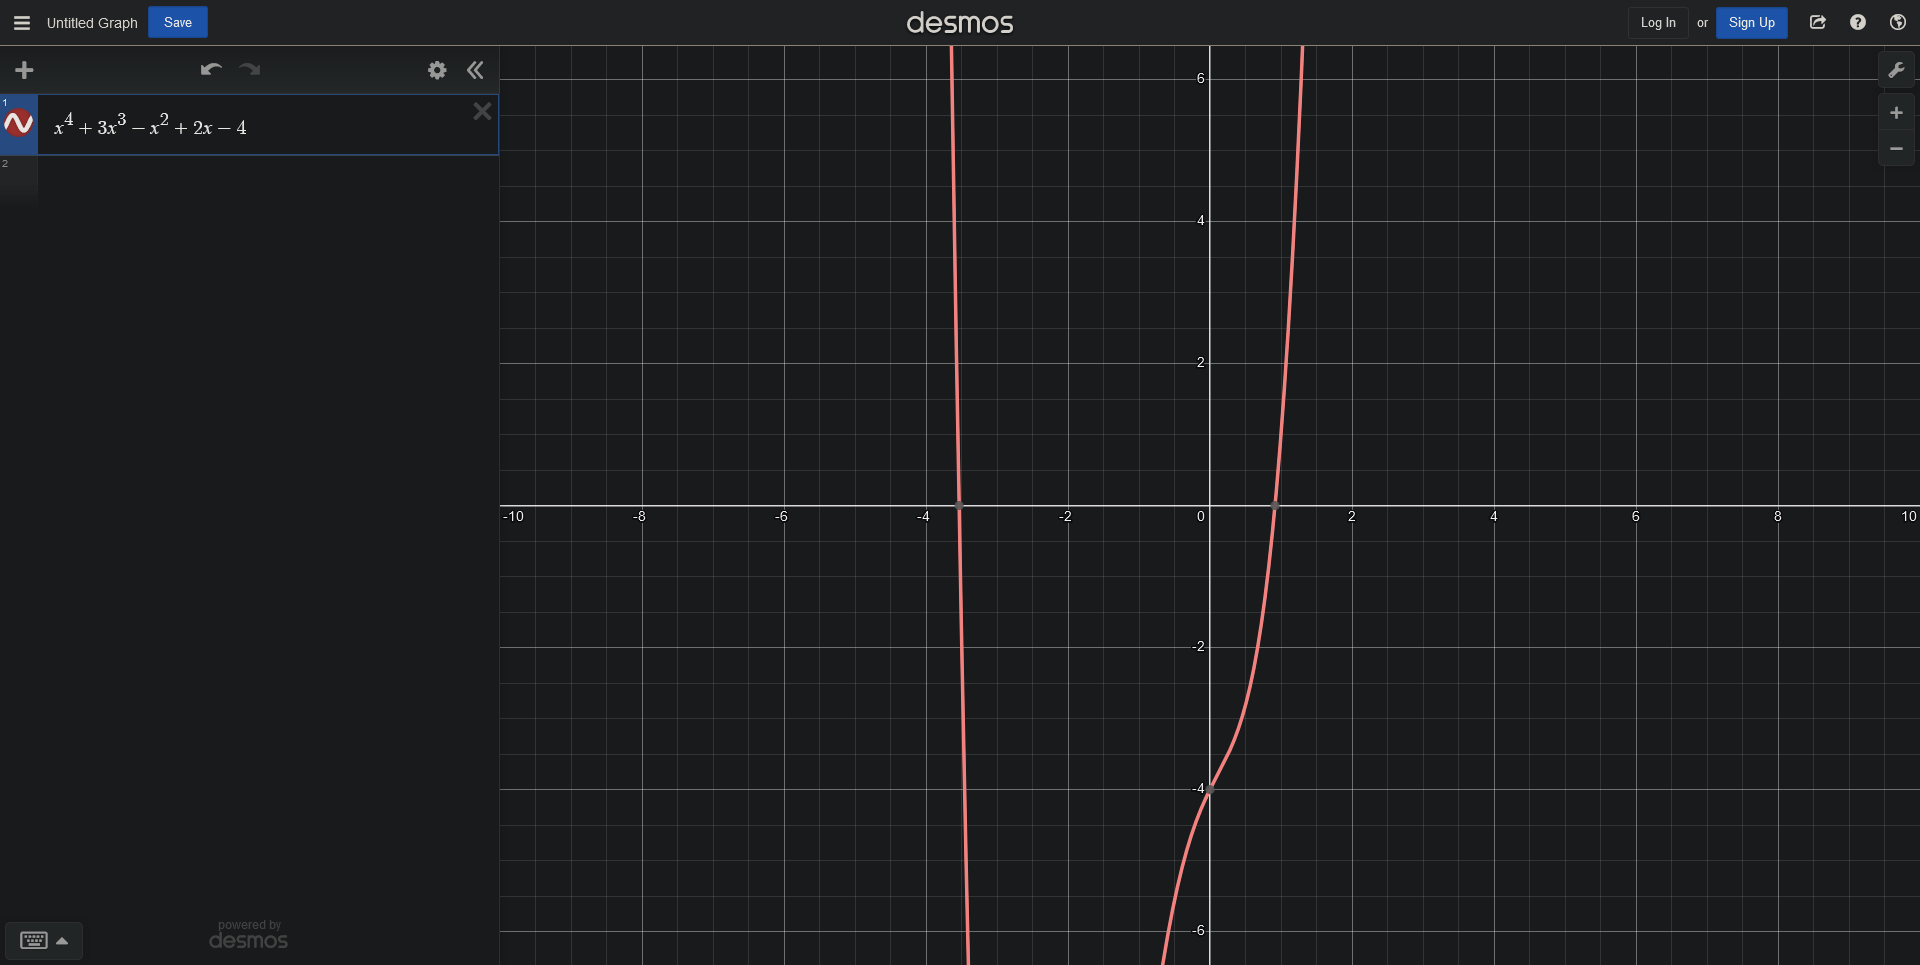
\includegraphics[scale=0.2]{gambar4.png}
        \end{center}
        Terlihat bahwa kurva memotong sumbu $ x $ di sekitar titik 1 dan -4. Maka akan dipilih 2 titik perkiraan awal $ x_0 $ yaitu $ x_0 = 1 $ dan $ x_0 = -3 $. Perhitungan hampiran akar akan dilakukan menggunakan bahasa pemograman "Rust" sebagai berikut
        \begin{lstlisting}[language=Rust, style=colouredRust]
    use std::io;

    // INPUT KE VARIABEL
    fn read() -> String {
        let mut buffer = String::new();
        io::stdin()
            .read_line(&mut buffer)
            .expect("Failed");
        return buffer;
    }

    // FUNGSI f(x)
    fn f(x:f64) -> f64{
        x.powi(4) + 3.0 * x.powi(3) - x.powi(2) + 2.0 * x - 4.0
    }

    // FUNGSI g(x)
    fn g(x:f64) -> f64 {
        (4.0 + x.powi(2) - 3.0 * x.powi(3) - x.powi(4)) / 2.0 // g1(x)
        (2.0 * x - 4.0 + 3.0 * x.powi(3) + x.powi(4)).sqrt() // g2(x)
        ((4.0 - 2.0 * x + x.powi(2) - x.powi(4)) / 3.0).cbrt() // g3(x)
        (4.0 - 2.0 * x + x.powi(2) - 3.0 * x.powi(3)).powf(0.25) // g4(x)
    }

    // ENTRY POINT
    fn main() {
        
        // INPUT X
        println!();
        println!("x = ");
        let mut x : f64 = read()
            .trim()
            .parse()
            .expect("Failed");

        // UJI PERKIRAAN AWAL
        if f(x) == 0.0 {
            println!();
            println!();
            println!("f(x) = {}", f(x));
            println!();
            println!("Solusi akhir = {x}");
            return ();
        }

        // INPUT GALAT
        println!();
        println!("Batas galat = ");
        let galat : f64 = read()
            .trim()
            .parse()
            .expect("Failed");

        // INPUT BATAS ITERASI
        println!();
        println!("Batas iterasi = ");
        let max : i32 = read()
            .trim()
            .parse()
            .expect("Failed");

        // LOOPING ALGORITMA
        let mut iter = 0;
        while   (true)
                & (f(g(x)) != 0.0) 
                & ((g(x) - x).abs() > galat) 
                & (iter < max){
            {
                // OUTPUT ITERASI
                println!();
                println!();
                println!("Iteras {iter}");
                println!();
                println!("x{iter} = {x}");
                println!("f(x{iter}) = {}",f(x));
                println!();
                println!("x{} = {}", iter + 1, g(x));
                println!("f(x{}) = {}", iter + 1, f(g(x)));
                println!();
                println!("galat = {}", ((g(x) - x) / g(x)).abs());
            }

            // PERHITUNGAN
            x = g(x);
            iter = iter + 1;
        }
        {
            // OUTPUT ITERASI
            println!();
            println!();
            println!("Iteras {iter}");
            println!();
            println!("x{iter} = {x}");
            println!("f(x{iter}) = {}",f(x));
            println!();
            println!("x{} = {}", iter + 1, g(x));
            println!("f(x{}) = {}", iter + 1, f(g(x)));
            println!();
            println!("galat = {}", ((g(x) - x) / g(x)).abs());
            println!();
            println!();
            println!("Solusi akhir = {x}");
        }
    }
        \end{lstlisting} 
        Perhitungan dilakukan dengan galat sebesar 0.00001 dan diperoleh hasil sebagai berikut
        \begin{enumerate}
            \item {
                Untuk $ g_1(x) $
                \begin{enumerate}
                    \item {
                        Untuk $ x_0 = 1 $
                        \begin{lstlisting}
    x =
    1
    
    Batas galat =
    0.00001
    
    Batas iterasi =
    1000
    
    
    Iteras 0
    
    x0 = 1
    f(x0) = 1
    
    x1 = 0.5
    f(x1) = -2.8125
    
    galat = 1
    
    
    Iteras 1
    
    x1 = 0.5
    f(x1) = -2.8125
    
    x2 = 1.90625
    f(x2) = 30.163865089416504
    
    galat = 0.7377049180327869
    
    .
    .
    .

    Iteras 7
    
    x7 = -47670310284984527000000000000000000000000000000000000000000000000000000000000000000000000000000000000000000000000000000000000000000000000000000000000000000000000000000000000000000000000000000000000000000000000000000000000000000000000000000000000000000000
    f(x7) = NaN
    
    x8 = NaN
    f(x8) = NaN
    
    galat = NaN
    
    
    Solusi akhir = -47670310284984527000000000000000000000000000000000000000000000000000000000000000000000000000000000000000000000000000000000000000000000000000000000000000000000000000000000000000000000000000000000000000000000000000000000000000000000000000000000000000000000
                        \end{lstlisting}
                        Diperoleh untuk $ x_0 = 1 $, perhitungan divergen
                    }
                    \item {
                        Untuk $ x_0 = -3 $
                        \begin{lstlisting}
    x =
    -3
    
    Batas galat =
    0.00001
    
    Batas iterasi =
    1000
    
    
    Iteras 0
    
    x0 = -3
    f(x0) = -19
    
    x1 = 6.5
    f(x1) = 2575.6875
    
    galat = 1.4615384615384615
    
    
    Iteras 1
    
    x1 = 6.5
    f(x1) = 2575.6875
    
    x2 = -1281.34375
    f(x2) = 2689331579209.2065
    
    galat = 1.0050727995512523
    
    .
    .
    .
    
    Iteras 5
    
    x5 = -3570094586357638000000000000000000000000000000000000000000000000000000000000000000000000000000000000000000000000000000000000000000000000000000000000000000000000000000000000000000000000000000000
    f(x5) = NaN
    
    x6 = NaN
    f(x6) = NaN
    
    galat = NaN
    
    
    Solusi akhir = -3570094586357638000000000000000000000000000000000000000000000000000000000000000000000000000000000000000000000000000000000000000000000000000000000000000000000000000000000000000000000000000000000
                        \end{lstlisting}
                        Diperoleh untuk $ x_0 = -3 $, perhitungan divergen
                    }
                \end{enumerate}
            }
            \item {
                Untuk $ g_2(x) $
                \begin{enumerate}
                    \item {
                        Untuk $ x_0 = 1 $
                        \begin{lstlisting}
    x =
    1
    
    Batas galat =
    0.00001
    
    Batas iterasi =
    1000
    
    
    Iteras 0
    
    x0 = 1
    f(x0) = 1
    
    x1 = 1.4142135623730951
    f(x1) = 9.313708498984761
    
    galat = 0.29289321881345254
    
    
    Iteras 1
    
    x1 = 1.4142135623730951
    f(x1) = 9.313708498984761
    
    x2 = 3.3635856610148585
    f(x2) = 233.57734586330625
    
    galat = 0.5795517923731427
    
    .
    .
    .
    
    Iteras 10
    
    x10 = inf
    f(x10) = NaN
    
    x11 = inf
    f(x11) = NaN
    
    galat = NaN
    
    
    Solusi akhir = inf
                        \end{lstlisting}
                        Diperoleh untuk $ x_0 = 1 $, perhitungan divergen
                    }
                    \item {
                        Untuk $ x_0 = -3 $
                        \begin{lstlisting}
    x =
    -3
    
    Batas galat =
    0.00001
    
    Batas iterasi =
    1000
    
    
    Iteras 0
    
    x0 = -3
    f(x0) = -19
    
    x1 = NaN
    f(x1) = NaN
    
    galat = NaN
    
    
    Solusi akhir = -3
                        \end{lstlisting}
                        Diperoleh untuk $ x_0 = -3 $ perhitungan divergen
                    }
                \end{enumerate}
            }
            \item {
                Untuk $ g_3(x) $ 
                \begin{enumerate}
                    \item {
                        Untuk $ x_0 = 1 $
                        \begin{lstlisting}
    x =
    1
    
    Batas galat =
    0.00001
    
    Batas iterasi =
    1000
    
    
    Iteras 0
    
    x0 = 1
    f(x0) = 1
    
    x1 = 0.8735804647362988
    f(x1) = -0.4335949224054252
    
    galat = 0.14471424255333196
    
    
    Iteras 1
    
    x1 = 0.8735804647362988
    f(x1) = -0.4335949224054252
    
    x2 = 0.93262920676064
    f(x2) = 0.1856033326436215
    
    galat = 0.06331427495117692
    
    .
    .
    .
    
    Iteras 12
    
    x12 = 0.9157548534009559
    f(x12) = 0.000039532295601496514
    
    x13 = 0.9157496155450033
    f(x13) = -0.00001697223888941224
    
    galat = 0.0000057197468211931175
    
    
    Solusi akhir = 0.9157548534009559
                        \end{lstlisting}
                        Diperoleh hasil akhir $ x = 0.9157548534009559 $
                    }
                    \item {
                        Untuk $ x_0 = -3 $
                        \begin{lstlisting}
    x =
    -3
    
    Batas galat =
    0.00001
    
    Batas iterasi =
    1000
    
    
    Iteras 0
    
    x0 = -3
    f(x0) = -19
    
    x1 = -2.7442487702296905
    f(x1) = -22.30492426861962
    
    galat = 0.09319535187362166
    
    
    Iteras 1
    
    x1 = -2.7442487702296905
    f(x1) = -22.30492426861962
    
    x2 = -2.3652213652991407
    f(x2) = -22.723910163170096
    
    galat = 0.16025028798207747
    
    .
    .
    .
    
    Iteras 17
    
    x17 = 0.9157549868296531
    f(x17) = 0.00004097169610517426
    
    x18 = 0.915749558259892
    f(x18) = -0.00001759021102865077
    
    galat = 0.000005928006966622007
    
    
    Solusi akhir = 0.9157549868296531
                        \end{lstlisting}
                        Diperoleh hasil akhir $ x = 0.9157549868296531 $
                    }
                \end{enumerate}
            }
            \item {
                Untuk $ g_4(x) $
                \begin{enumerate}
                    \item {
                        Untuk $ x_0 = 1 $ 
                        \begin{lstlisting}
    x =
    1
    
    Batas galat =
    0.00001
    
    Batas iterasi =
    1000
    
    
    Iteras 0
    
    x0 = 1
    f(x0) = 1
    
    x1 = 0
    f(x1) = -4
    
    galat = inf
    
    
    Iteras 1
    
    x1 = 0
    f(x1) = -4
    
    x2 = 1.4142135623730951
    f(x2) = 9.313708498984761
    
    galat = 1
    
    
    Iteras 2
    
    x2 = 1.4142135623730951
    f(x2) = 9.313708498984761
    
    x3 = NaN
    f(x3) = NaN
    
    galat = NaN
    
    
    Solusi akhir = 1.4142135623730951
                        \end{lstlisting}
                        Diperoleh untuk $ x_0 = 1 $ perhitungan divergen
                    }
                    \item {
                        Untuk $ x_0 = -3 $
                        \begin{lstlisting}
    x =
    -3
    
    Batas galat =
    0.00001
    
    Batas iterasi =
    1000
    
    
    Iteras 0
    
    x0 = -3
    f(x0) = -19
    
    x1 = 3.1622776601683795
    f(x1) = 187.1928851253882
    
    galat = 1.948683298050514
    
    
    Iteras 1
    
    x1 = 3.1622776601683795
    f(x1) = 187.1928851253882
    
    x2 = NaN
    f(x2) = NaN
    
    galat = NaN
    
    
    Solusi akhir = 3.1622776601683795
                        \end{lstlisting}
                        Diperoleh untuk $ x_0 = -3 $ perhitungan divergen
                    }
                \end{enumerate}
            }
            \item {
                Untuk $ g_5(x) $

                Untuk fungsi $ g_5(x) $, perhitungan dilakukan dengan \emph{software} Microsoft Excel sebagai berikut
                \begin{longtable}[c]{|l|l|l|l|}
                    \hline
                    r & Xr                & |X(r+1)-Xr|          & 0.0001 \\ \hline
                    \endfirsthead
                    %
                    \endhead
                    %
                    0 & 0.01              &                      &        \\ \hline
                    1 & 1.09759595055116  & 1.08759595055116     & Lanjut \\ \hline
                    2 & 0.902241791682542 & 0.195354158868614    & Lanjut \\ \hline
                    3 & 0.917056548580811 & 0.0148147568982694   & Lanjut \\ \hline
                    4 & 0.915627300573917 & 0.0014292480068937   & Lanjut \\ \hline
                    5 & 0.915762967278311 & 0.000135666704394133 & Lanjut \\ \hline
                    6 & 0.915750069217386 & 1.28980609249707E-05 & Stop   \\ \hline
                \end{longtable}
                Diperoleh hasil akhir $ x = 0.915750069217386 $
            }
            \item {
                Untuk $ g_6(x) $

                Untuk fungsi $ g_6(x) $, perhitungan dilakukan dengan \emph{software} Microsoft Excel sebagai berikut
                \begin{longtable}[c]{|l|l|l|l|}
                    \hline
                    r  & Xr                & |X(r+1)-Xr|          & 0.0001 \\ \hline
                    \endfirsthead
                    %
                    \endhead
                    %
                    0  & -3                &                      &        \\ \hline
                    1  & -3.21829794868543 & 0.218297948685432    & Lanjut \\ \hline
                    2  & -3.34816164111402 & 0.129863692428589    & Lanjut \\ \hline
                    3  & -3.42488677671783 & 0.0767251356038079   & Lanjut \\ \hline
                    4  & -3.470012011725   & 0.0451252350071729   & Lanjut \\ \hline
                    5  & -3.49647797695354 & 0.026465965228534    & Lanjut \\ \hline
                    6  & -3.51197425362695 & 0.0154962766734186   & Lanjut \\ \hline
                    7  & -3.52103856884729 & 0.00906431522033691  & Lanjut \\ \hline
                    8  & -3.52633749911181 & 0.00529893026451944  & Lanjut \\ \hline
                    9  & -3.52943414885049 & 0.00309664973867774  & Lanjut \\ \hline
                    10 & -3.53124344020269 & 0.00180929135220342  & Lanjut \\ \hline
                    11 & -3.53230043722413 & 0.00105699702143847  & Lanjut \\ \hline
                    12 & -3.53291789761792 & 0.000617460393789404 & Lanjut \\ \hline
                    13 & -3.53327858169092 & 0.000360684072999273 & Lanjut \\ \hline
                    14 & -3.53348926717297 & 0.00021068548205383  & Lanjut \\ \hline
                    15 & -3.53361233266363 & 0.000123065490652774 & Lanjut \\ \hline
                    16 & -3.53368421703493 & 7.18843713003459E-05 & Stop   \\ \hline
                \end{longtable}
                Diperoleh hasil akhir $ x = -3.53368421703493 $
            }
        \end{enumerate}
        Dari semua kemungkinan, diperoleh
        \begin{enumerate}
            \item fungsi $ g_3(x) $ dengan $ x_0 = 1 $ konvergen dan diperoleh hasil akhir $ x = 0.9157511353924488 $
            \item fungsi $ g_3(x) $ dengan $ x_0 = -3 $ konvergen dan diperoleh hasil akhir $ x = 0.9157549868296531 $
            \item fungsi $ g_5(x) $ dengan $ x_0 = 1 $ konvergen dan diperoleh hasil akhir $ x = 0.915750069217386 $
            \item fungsi $ g_6(x) $ dengan $ x_0 = -3 $ konvergen dan diperoleh hasil akhir $ x = -3.53368421703493 $
        \end{enumerate}
    }
    \item {
        Apa yang dapat kalian simpulkan mengenai kelebihan dan kekurangan metode iterasi titik tetap dibandingkan dengan metode-metode lain yang digunakan untuk menentukan hampiran akar persamaan tak linier? Jelaskan!
        \begin{enumerate}
            \item {
                Kelebihan
                \begin{enumerate}
                    \item Algoritma yang digunakan lebih mudah jika dibandingkan dengan metode sebelumnya
                \end{enumerate}
            }
            \item {
                Kekurangan
                \begin{enumerate}
                    \item Proses iterasi yang tidak efisien
                    \item Tidak dapat digunakan untuk semua fungsi
                    \item Nilai $x$ saat iterasi dapat menjauhi nilai hampiran akar $x$ sebenarnya
                    \item Jika $f(x)$ mempunyai beberapa akar, maka akar tersebut tidak dapat dicari secara langsung atau bersamaan
                    \item Tidak dapat mencari akar kompleks
                    \item Jika persamaan non linear cukup rumit, akan sulit untuk mencari turunan $g(x)$ (untuk mencari kekonvergenan)
                \end{enumerate}
            }
        \end{enumerate}
        \qquad Jika dilihat dari soal nomor 1, iterasi yang diperlukan untuk mendapatkan hampiran akar sama atau lebih sedikit dari metode-metode sebelumnya. Namun perbandingan ini tidak begitu menggambarkan perbedaan metode-metode ini karena pengambilan titik perkiraan awal $ x_0 $ pada metode iterasi titik tetap bergantung pada pemilihan fungsi $ g(x) $ yang akan digunakan. Selain itu, metode iterasi titik tetap menjamin kekonvergenan jika titik perkiraan awal $ x_0 $ diambil dari interval dimana $ |g'(x)| < 1 $. Tetapi terkadang menentukan solusi untuk $ |g'(x)| < 1 $ tidak dapat dilakukan sehingga menentukan fungsi $ g(x) $ yang akan digunakan harus dilakukan dengan mencoba-coba. Metode ini sangatlah fleksibel tapi karena fleksibelnya itu cukup susah untuk menemukan hampiran akar karena terlalu banyak kemungkinan persamaan yg dapat dibuat. 
    }
\end{enumerate}

\end{document}